\documentclass[aspectratio=169]{beamer}
\usepackage{amsmath}
\usepackage{amssymb}
\usepackage{xcolor}
\usepackage{cancel}
\usepackage{tikz}
\usetikzlibrary{arrows.meta,decorations.pathreplacing}

% ================================================================
% Quick Questions deck: introducing algebra, for a Year 7 class
% meeting algebra for the first time.
%
% Each topic opens with five true/false statements and then runs ten
% quick questions that get gradually harder. Every question gets two
% slides: the question on its own for the mini whiteboards, then the
% same question again with the solution underneath in red.
%
% The three green topics are algebraic notation, the vocabulary of
% algebra (variable, coefficient, constant, term, expression) and
% simplifying expressions with one variable. The three amber topics
% simplify expressions with more than one variable and with non-linear
% terms, then multiply and divide variables using index notation. The
% three red topics write expressions for real-life situations,
% simplify expressions with negative powers, and multiply and divide
% algebraic expressions.
%
% Where the working can be drawn it is: a labelled expression for the
% vocabulary; bar models for collecting like terms and for the
% real-life situations; algebra tiles to show that x^2 and x are not
% like terms; area models for multiplying; crossing out common factors
% for dividing; and a ladder of powers that divides by x at every step,
% for the negative powers. Questions whose answer is the whole of the
% working show only the answer, at the same size as the question.
% ================================================================

\setbeamertemplate{navigation symbols}{}

% A link in the bottom left of every slide back to the contents, so a
% deck this long can be jumped around in during a lesson.
\setbeamertemplate{footline}{%
  \hbox to\paperwidth{%
    \hspace{1em}%
    \hyperlink{contents}{%
      \color{gray}\scriptsize$\leftarrow$~Back to contents}%
    \hfil}%
  \vskip4pt%
}

% An expression is never broken across two lines. If one is too wide
% for the slide it shows up as an overfull box in the log, and the
% size is dropped for that question.
\binoppenalty=10000
\relpenalty=10000

% Topic divider.
\newcommand{\qtopic}[1]{%
  \section{#1}%
  \begin{frame}
    \vfill
    \begin{center}
      {\usebeamercolor[fg]{structure}\Huge\bfseries #1}
    \end{center}
    \vfill
  \end{frame}%
}

% \qq[<question size>][<solution size>]{<question>}{<solution>}
% The two optional sizes drop the type for the wordier questions and
% the longer solutions, so nothing runs off the slide.
\NewDocumentCommand{\qq}{O{\Huge}O{\LARGE}+m+m}{%
  \begin{frame}
    \vfill
    \begin{center}
      \begin{minipage}{0.92\textwidth}
        \centering #1 #3
      \end{minipage}
    \end{center}
    \vfill
  \end{frame}%
  \begin{frame}
    \vfill
    \begin{center}
      \begin{minipage}{0.92\textwidth}
        \centering #1 #3
        \par\vspace{0.9em}
        {\color{red}#2 #4}
      \end{minipage}
    \end{center}
    \vfill
  \end{frame}%
}

% \tf[<statement size>][<answer size>]{<statement>}{<answer>}
% As \qq, but with a standing "True or false?" heading above the
% statement. The statements hunt for the usual misconceptions, so the
% answer says why, not just which.
\NewDocumentCommand{\tf}{O{\LARGE}O{\Large}+m+m}{%
  \begin{frame}
    \vfill
    \begin{center}
      \begin{minipage}{0.92\textwidth}
        \centering
        {\usebeamercolor[fg]{structure}\Large\bfseries True or false?}
        \par\vspace{1em}
        #1 #3
      \end{minipage}
    \end{center}
    \vfill
  \end{frame}%
  \begin{frame}
    \vfill
    \begin{center}
      \begin{minipage}{0.92\textwidth}
        \centering
        {\usebeamercolor[fg]{structure}\Large\bfseries True or false?}
        \par\vspace{1em}
        #1 #3
        \par\vspace{0.9em}
        {\color{red}#2 #4}
      \end{minipage}
    \end{center}
    \vfill
  \end{frame}%
}

% \qa[<size>]{<question>}{<answer>}
% The answer-only version of \qq: one size sets both the question and
% the answer, so the answer is in the same font.
\NewDocumentCommand{\qa}{O{\Huge}+m+m}{\qq[#1][#1]{#2}{#3}}

% \ans{<answer>} sets the final answer of a worked solution on a line
% of its own at the size of the questions, so that it stands out from
% the working or the reason written beside it.
\newcommand{\ans}[1]{{\Huge #1\par}}

% The wording of the questions. \notn, \indexq and \termq put the
% instruction on its own line in a smaller size, so that the
% expression underneath can be as large as possible.
\newcommand{\simp}[1]{Simplify $#1$}
\newcommand{\notn}[1]{{\LARGE Write in algebraic notation}\par\vspace{0.4em}$#1$}
\newcommand{\indexq}[1]{{\LARGE Write using index notation}\par\vspace{0.4em}$#1$}
\newcommand{\termq}[2]{$#1$\par\vspace{0.4em}{\LARGE #2}}

% Chained working, one equation per row, with the equals signs lined
% up. \dfrac is taller than the row strut, so rows with a fraction
% carry an explicit skip such as \\[0.95em].
\newcommand{\work}[1]{%
  \begin{tabular}{@{}r@{\;=\;}l@{}}#1\end{tabular}%
}

% \side[<width of the left part>]{<left>}{<right>}
% Two pieces of a solution next to each other, for a solution that
% would be too tall with one above the other.
\NewDocumentCommand{\side}{O{0.5}+m+m}{%
  \begin{minipage}[c]{#1\linewidth}\centering #2\end{minipage}\hfill
  \begin{minipage}[c]{\dimexpr0.98\linewidth-#1\linewidth\relax}%
    \centering #3\end{minipage}%
}

% ================================================================
% Pictures
% ================================================================

\tikzset{
  bx/.style={draw=red!60!black, thick},
  blab/.style={text=red, font=\Large, inner sep=1pt},
  brc/.style={decorate, decoration={brace, amplitude=6pt, raise=2pt},
              red, thick},
  brcd/.style={decorate, decoration={brace, amplitude=6pt, raise=2pt,
               mirror}, red, thick},
}

% Bar models. Inside a tikzpicture:
% \brow[<name>]{<y>}{<row label>}{<label>/<width in cm>/<fill>, ...}
% draws one row of bars 0.9 cm tall, centred on height <y> and
% starting at x=0, with the row label (which can be empty) to the
% left. A variable keeps the same width and fill everywhere in a
% picture, so bars of different variables are visibly different
% lengths and cannot be counted together.
% Each bar leaves two coordinates, <name>l<k> and <name>r<k>, at the
% middle of its left and right edges, where k counts the bars from 1.
% \bup[<name>]{<first bar>}{<last bar>}{<label>} and \bdown draw a
% labelled brace above or below a run of bars in that row.
\NewDocumentCommand{\brow}{O{b}mmm}{%
  \if\relax\detokenize{#3}\relax\else
    \node[blab, anchor=east] at (-0.25,#2) {#3};%
  \fi
  \gdef\bx{0}%
  \foreach \lab/\w/\f [count=\k] in {#4}{%
    \draw[bx, fill=\f] (\bx,{#2-0.45}) rectangle ++(\w,0.9);
    \node[blab] at ({\bx+\w/2},#2) {$\lab$};
    \coordinate (#1l\k) at (\bx,#2);
    \coordinate (#1r\k) at ({\bx+\w},#2);
    \pgfmathsetmacro{\nx}{\bx+\w}%
    \xdef\bx{\nx}%
  }%
}
\NewDocumentCommand{\bup}{O{b}mmm}{%
  \draw[brc] ([yshift=0.45cm]#1l#2) -- ([yshift=0.45cm]#1r#3)
    node[midway, above=9pt, blab] {#4};}
\NewDocumentCommand{\bdown}{O{b}mmm}{%
  \draw[brcd] ([yshift=-0.45cm]#1l#2) -- ([yshift=-0.45cm]#1r#3)
    node[midway, below=9pt, blab] {#4};}

% Algebra tiles. Inside a tikzpicture:
% \tilerow[<side of the square in cm>]{<letter>}{<list of s and r>}
% s is a square tile, <letter> by <letter>, so its area is <letter>^2.
% r is a rectangle, <letter> by 1, so its area is <letter>. The tiles
% stand side by side along y=0 with a small gap between them. The
% side of the square is not a whole number of the short side of the
% rectangle, because the variable can stand for any number.
% Each tile leaves coordinates tl<k> and tr<k> at its bottom-left and
% bottom-right corners, and \tbrace{<first tile>}{<last tile>}{<label>}
% draws a labelled brace underneath a run of tiles.
\NewDocumentCommand{\tilerow}{O{1.6}mm}{%
  \gdef\tx{0}%
  \foreach \tk [count=\k] in {#3}{%
    \if s\tk \def\tkW{#1}\def\tkF{red!25}\def\tkL{#2^{2}}\fi
    \if r\tk \pgfmathsetmacro{\tkW}{0.34*#1}\def\tkF{red!8}\def\tkL{#2}\fi
    \draw[bx, fill=\tkF] (\tx,0) rectangle ++(\tkW,#1);
    \node[blab] at ({\tx+\tkW/2},{#1/2}) {$\tkL$};
    \coordinate (tl\k) at (\tx,0);
    \coordinate (tr\k) at ({\tx+\tkW},0);
    \pgfmathsetmacro{\nx}{\tx+\tkW+0.15}%
    \xdef\tx{\nx}%
  }%
}
\newcommand{\tbrace}[3]{%
  \draw[brcd] ([yshift=-0.05cm]tl#1) -- ([yshift=-0.05cm]tr#2)
    node[midway, below=9pt, blab] {#3};}

% \areamodel[<cell width>][<cell height>]{<rows>}{<row label>}{<columns>}{<column label>}{<cell label>}
% A rectangle split into a grid, with the length of each row written
% down the left and the length of each column written along the top.
% Each cell is one row length times one column length, so counting the
% cells gives the product.
\NewDocumentCommand{\areamodel}{O{1.0}O{0.7}mmmmm}{%
  \begin{tikzpicture}[baseline=(current bounding box.center)]
    \foreach \i in {1,...,#3}{%
      \node[blab, anchor=east] at (-0.1,{-(\i-0.5)*#2}) {$#4$};}
    \foreach \j in {1,...,#5}{%
      \node[blab, anchor=south] at ({(\j-0.5)*#1},0.08) {$#6$};
      \foreach \i in {1,...,#3}{%
        \draw[bx, fill=red!8] ({(\j-1)*#1},{-(\i-1)*#2}) rectangle ++(#1,-#2);
        \node[blab, font=\large] at ({(\j-0.5)*#1},{-(\i-0.5)*#2}) {$#7$};}}
  \end{tikzpicture}%
}

% \anatomy{<coefficient>}{<variable>}{<constant term, with its sign>}
% An expression of the form 5x+3 with each part labelled. The constant
% is labelled together with its sign, because the sign in front of a
% term belongs to the term.
\newcommand{\anatomy}[3]{%
  \begin{tikzpicture}[baseline=(v.base),
      part/.style={inner xsep=0pt, inner ysep=2pt, text=red, font=\Huge,
                   text height=0.75em, text depth=0.25em},
      lab/.style={text=red, font=\Large, inner sep=2pt},
      arr/.style={-{Stealth[length=7pt]}, red, thick, shorten >=3pt}]
    \node[part] (c) {$#1$};
    \node[part, anchor=base west] (v) at (c.base east) {$#2$};
    \node[part, anchor=base west] (k) at ([xshift=8pt]v.base east) {$#3$};
    \node[lab, anchor=east] (cl) at ([xshift=-1.2cm]c.west) {coefficient};
    \draw[arr] (cl.east) -- (c.west);
    \node[lab] (vl) at ([yshift=1.0cm]v.north) {variable};
    \draw[arr] (vl.south) -- (v.north);
    \node[lab, anchor=west] (kl) at ([xshift=1.2cm]k.east) {constant};
    \draw[arr] (kl.west) -- (k.east);
    \draw[brcd] (c.south west) -- (k.south east)
      node[midway, below=10pt, lab] {expression};
  \end{tikzpicture}%
}

% The powers of x running down from x^3 to x^{-2}, dividing by x at
% every step. The negative powers are not a new rule: they are the same
% pattern carried on past x^0=1.
\newcommand{\xladder}{%
  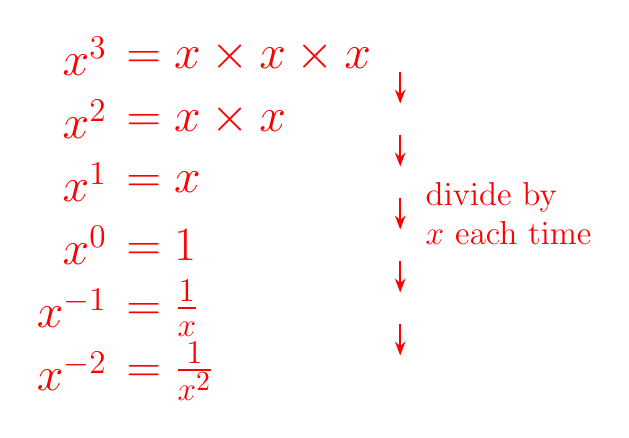
\begin{tikzpicture}[x=1cm,y=1cm,text=red,font=\LARGE]
    \node[anchor=east] at (0,0)    {$x^{3}$};  \node[anchor=west] at (0,0)    {$=x\times x\times x$};
    \node[anchor=east] at (0,-0.8) {$x^{2}$};  \node[anchor=west] at (0,-0.8) {$=x\times x$};
    \node[anchor=east] at (0,-1.6) {$x^{1}$};  \node[anchor=west] at (0,-1.6) {$=x$};
    \node[anchor=east] at (0,-2.4) {$x^{0}$};  \node[anchor=west] at (0,-2.4) {$=1$};
    \node[anchor=east] at (0,-3.2) {$x^{-1}$}; \node[anchor=west] at (0,-3.2) {$=\frac{1}{x}$};
    \node[anchor=east] at (0,-4.0) {$x^{-2}$}; \node[anchor=west] at (0,-4.0) {$=\frac{1}{x^{2}}$};
    \foreach \i in {0,...,4}{%
      \draw[-{Stealth[length=5pt]},red,thick] (3.6,{-0.8*\i-0.2}) -- (3.6,{-0.8*\i-0.6});}
    \node[anchor=west,font=\large,align=left] at (3.8,-2.0) {divide by\\ $x$ each time};
  \end{tikzpicture}%
}

% \rectlab[<colour>]{<length label>}{<width label>}
% A rectangle with its length written underneath and its width on the
% left. Black when it is part of the question, red in a solution.
\NewDocumentCommand{\rectlab}{O{black}mm}{%
  \begin{tikzpicture}[baseline=(current bounding box.center)]
    \draw[thick, draw=#1] (0,0) rectangle (4.2,1.6);
    \node[below, text=#1, font=\LARGE] at (2.1,0) {$#2$};
    \node[left, text=#1, font=\LARGE] at (0,0.8) {$#3$};
  \end{tikzpicture}%
}

% Contents-slide bullets, colour-coded by difficulty band: green for
% notation, vocabulary and one variable; orange for more than one
% variable, non-linear terms and index notation; red for real-life
% situations, negative powers and multiplying and dividing
% expressions. The green is darkened because a pure green washes out
% on a projector.
\setbeamertemplate{section in toc}{%
  \ifnum\inserttocsectionnumber<4
    \textcolor{green!55!black}{$\bullet$}%
  \else
    \ifnum\inserttocsectionnumber<7
      \textcolor{orange}{$\bullet$}%
    \else
      \textcolor{red}{$\bullet$}%
    \fi
  \fi
  ~\inserttocsection%
}

\title{Introducing Algebra: Quick Questions}
\subtitle{Mini whiteboard questions, with solutions}
\author{}
\date{}

\begin{document}

\frame{\titlepage}

\begin{frame}[label=contents]{Contents}
  \small
  \tableofcontents
\end{frame}

%================================================================
\qtopic{Algebraic notation}
%================================================================

\tf{$3a$ means $3+a$}
  {\textbf{False.} $3a$ means $3\times a$.\\[0.3em]
   When $a=2$, $3a=6$ but $3+a=5$.}

\tf{$a\times b$ is written as $ab$}
  {\textbf{True.} In algebra we leave out the multiplication sign.}

\tf{$4\times y$ is written as $y4$}
  {\textbf{False.} The number is written in front of the letter.\\[0.3em]
   $4\times y=4y$}

\tf{$m\div 5$ is written as $\dfrac{m}{5}$}
  {\textbf{True.} In algebra we write a division as a fraction.}

\tf{$2\times(x+1)$ is written as $2x+1$}
  {\textbf{False.} The $2$ multiplies all of $x+1$, so the bracket stays.\\[0.3em]
   $2\times(x+1)=2(x+1)$}

\qa{\notn{5\times x}}{$5x$}

\qq{\notn{y\times 7}}
  {\ans{$7y$}\vspace{0.3em}
   The number is written in front of the letter.}

\qa{\notn{a\times b}}{$ab$}

\qq{\notn{1\times n}}
  {\ans{$n$}\vspace{0.3em}
   One lot of $n$ is $n$, so we do not write the $1$.}

\qa{\notn{p\div 3}}{$\dfrac{p}{3}$}

\qq{\notn{b\times 2\times a}}
  {\ans{$2ab$}\vspace{0.3em}
   The number goes first,\\ then the letters in alphabetical order.}

\qa{\notn{x\times 4+1}}{$4x+1$}

\qa{\notn{(m+2)\div 5}}{$\dfrac{m+2}{5}$}

\qa{\notn{3\times(y-4)}}{$3(y-4)$}

\qa{{\LARGE Write using $\times$ and $\div$ signs}\par\vspace{0.4em}$\dfrac{3a}{4}$}
  {$3\times a\div 4$}

%================================================================
\qtopic{Algebraic terminology}
%================================================================

\tf{$3a+5$ is an equation}
  {\textbf{False.} $3a+5$ has no equals sign, so it is an expression.\\[0.3em]
   $3a+5=11$ is an equation.}

\tf{In $6y+2$, the coefficient of $y$ is $6$}
  {\textbf{True.} The coefficient is the number in front of the variable.
   \par\vspace{0.5em}
   \anatomy{6}{y}{+2}}

\tf{In $x+9$, the coefficient of $x$ is $0$}
  {\textbf{False.} $x$ means $1x$, one lot of $x$.\\[0.3em]
   The coefficient of $x$ is $1$.}

\tf{$2x+3y+4$ has three terms}
  {\textbf{True.} The terms are $2x$, $3y$ and $4$.}

\tf{In $5m-8$, the constant is $8$}
  {\textbf{False.} The constant is $-8$. The sign in front of a term\\
   belongs to the term.
   \par\vspace{0.5em}
   \anatomy{5}{m}{-8}}

\qq[\Huge][\Large]{\termq{4y+3}{What is the variable?}}
  {\ans{$y$}\vspace{0.3em}
   \anatomy{4}{y}{+3}}

\qa{\termq{7x+2}{What is the coefficient of $x$?}}{$7$}

\qa{\termq{5a+9}{What is the constant?}}{$9$}

\qq{\termq{3p+2q+1}{How many terms are there?}}
  {\ans{$3$}\vspace{0.3em}
   The terms are $3p$, $2q$ and $1$.}

\qq{\termq{2n+5=11}{Is this an expression or an equation?}}
  {\ans{An equation}\vspace{0.3em}
   It has an equals sign.}

\qq{\termq{m+6}{What is the coefficient of $m$?}}
  {\ans{$1$}\vspace{0.3em}
   $m$ means $1m$, one lot of $m$.}

\qq[\Huge][\Large]{\termq{4y-7}{What is the constant?}}
  {\ans{$-7$}\vspace{0.3em}
   \anatomy{4}{y}{-7}}

\qa{\termq{6x-2y+5}{Write down the terms}}{$6x$,\quad $-2y$,\quad $5$}

\qq{\termq{8-3t}{What is the coefficient of $t$?}}
  {\ans{$-3$}\vspace{0.3em}
   The term in $t$ is $-3t$.}

\qa[\LARGE]{Write an expression with variable $n$,\\[0.2em]
   coefficient $5$ and constant $-2$}
  {{\Huge $5n-2$}}

%================================================================
\qtopic{Simplifying expressions with one variable}
%================================================================

\tf{$a+a+a=a^{3}$}
  {\textbf{False.} $a+a+a$ is three lots of $a$, so $a+a+a=3a$.\\[0.3em]
   $a^{3}$ means $a\times a\times a$.
   \par\vspace{0.4em}
   \begin{tikzpicture}
     \brow{0}{}{a/1.8/red!8,a/1.8/red!8,a/1.8/red!8}
     \bdown{1}{3}{$3a$}
   \end{tikzpicture}}

\tf{$2y+3y=5y$}
  {\textbf{True.} Two lots of $y$ add three lots of $y$ is five lots of $y$.}

\tf{$5x-x=5$}
  {\textbf{False.} $x$ means $1x$.\\[0.3em]
   $5x-x=5x-1x=4x$}

\tf{$4m+3=7m$}
  {\textbf{False.} $4m$ and $3$ are not like terms,\\
   so $4m+3$ cannot be simplified.}

\tf{$3x-7x=-4x$}
  {\textbf{True.} $3-7=-4$, so $3x-7x=-4x$.}

\qq[\Huge][\Huge]{\simp{a+a+a+a}}
  {$4a$
   \par\vspace{0.4em}
   \begin{tikzpicture}
     \brow{0}{}{a/1.8/red!8,a/1.8/red!8,a/1.8/red!8,a/1.8/red!8}
     \bdown{1}{4}{$4a$}
   \end{tikzpicture}}

\qq[\Huge][\Huge]{\simp{3x+5x}}
  {$8x$
   \par\vspace{0.4em}
   \begin{tikzpicture}
     \brow{0}{}{x/1.3/red!25,x/1.3/red!25,x/1.3/red!25,x/1.3/red!8,x/1.3/red!8,x/1.3/red!8,x/1.3/red!8,x/1.3/red!8}
     \bup{1}{3}{$3x$}
     \bup{4}{8}{$5x$}
     \bdown{1}{8}{$8x$}
   \end{tikzpicture}}

\qa{\simp{9y-4y}}{$5y$}

\qa{\simp{n+6n}}{$7n$}

\qa{\simp{7p-p}}{$6p$}

\qa{\simp{2a+4a+3a}}{$9a$}

\qa{\simp{8x-3x+5x}}{$10x$}

\qa{\simp{4x-9x}}{$-5x$}

\qq{\simp{5y+3+2y}}
  {\ans{$7y+3$}\vspace{0.3em}
   $5y$ and $2y$ are like terms. The $3$ is not.}

\qa{\simp{6t+4-2t-9}}{$4t-5$}

%================================================================
\qtopic{Simplifying expressions with more than one variable}
%================================================================

\tf{$2a+3b=5ab$}
  {\textbf{False.} $2a$ and $3b$ are not like terms,\\
   so $2a+3b$ cannot be simplified.
   \par\vspace{0.4em}
   \begin{tikzpicture}
     \brow{0}{}{a/1.8/red!8,a/1.8/red!8,b/1.0/red!25,b/1.0/red!25,b/1.0/red!25}
     \bup{1}{2}{$2a$}
     \bup{3}{5}{$3b$}
   \end{tikzpicture}}

\tf{$4x+2y+x=5x+2y$}
  {\textbf{True.} $4x$ and $x$ are like terms: $4x+x=5x$.}

\tf{$a+b+a+b=a^{2}+b^{2}$}
  {\textbf{False.} $a+a$ is two lots of $a$, which is $2a$.\\[0.3em]
   $a+b+a+b=2a+2b$}

\tf{$3ab+2ba=5ab$}
  {\textbf{True.} $ba$ is the same as $ab$, because $b\times a=a\times b$.}

\tf{$5p-2q=3pq$}
  {\textbf{False.} $5p$ and $2q$ are not like terms,\\
   so $5p-2q$ cannot be simplified.}

\qq[\Huge][\Huge]{\simp{3a+2b+a+4b}}
  {$4a+6b$
   \par\vspace{0.4em}
   \begin{tikzpicture}
     \brow[p]{0}{}{a/1.3/red!8,a/1.3/red!8,a/1.3/red!8,b/0.75/red!25,b/0.75/red!25,a/1.3/red!8,b/0.75/red!25,b/0.75/red!25,b/0.75/red!25,b/0.75/red!25}
     \brow[q]{-1.3}{}{a/1.3/red!8,a/1.3/red!8,a/1.3/red!8,a/1.3/red!8,b/0.75/red!25,b/0.75/red!25,b/0.75/red!25,b/0.75/red!25,b/0.75/red!25,b/0.75/red!25}
     \bdown[q]{1}{4}{$4a$}
     \bdown[q]{5}{10}{$6b$}
   \end{tikzpicture}}

\qa{\simp{5x+3y+2x+y}}{$7x+4y$}

\qa{\simp{6m+4n-2m}}{$4m+4n$}

\qa{\simp{7p+3q-4p-q}}{$3p+2q$}

\qa{\simp{2a+5+3b+4a-2}}{$6a+3b+3$}

\qa{\simp{4x-3y+2x+5y}}{$6x+2y$}

\qq{\simp{5ab+2ab-3a}}
  {\ans{$7ab-3a$}\vspace{0.3em}
   $ab$ and $a$ are not like terms.}

\qq{\simp{4xy+3yx-2x}}
  {\ans{$7xy-2x$}\vspace{0.3em}
   $yx$ is the same as $xy$.}

\qa{\simp{3c-5d-4c+2d}}{$-c-3d$}

\qq[\LARGE][\LARGE]{Write an expression for the perimeter\\[0.2em] of this rectangle.
   \par\vspace{0.5em}
   \rectlab{2a+b}{a}}
  {$2a+b+a+2a+b+a$
   \par\vspace{0.4em}
   \ans{$6a+2b$}}

%================================================================
\qtopic{Simplifying expressions with non-linear terms}
%================================================================

\tf{$x^{2}+x^{2}=x^{4}$}
  {\textbf{False.} $x^{2}+x^{2}$ is two lots of $x^{2}$, so $x^{2}+x^{2}=2x^{2}$.\\[0.3em]
   $x^{4}$ means $x\times x\times x\times x$.
   \par\vspace{0.4em}
   \begin{tikzpicture}
     \tilerow{x}{s,s}
     \tbrace{1}{2}{$2x^{2}$}
   \end{tikzpicture}}

\tf{$5a^{2}-2a^{2}=3a^{2}$}
  {\textbf{True.} $5a^{2}$ and $2a^{2}$ are like terms: $5-2=3$.}

\tf{$3x^{2}+2x=5x^{3}$}
  {\textbf{False.} $x^{2}$ and $x$ are not like terms,\\
   so $3x^{2}+2x$ cannot be simplified.
   \par\vspace{0.4em}
   \begin{tikzpicture}
     \tilerow{x}{s,s,s,r,r}
     \tbrace{1}{3}{$3x^{2}$}
     \tbrace{4}{5}{$2x$}
   \end{tikzpicture}}

\tf{$y^{3}+y^{3}+y^{3}=3y^{3}$}
  {\textbf{True.} $y^{3}+y^{3}+y^{3}$ is three lots of $y^{3}$.}

\tf{$a^{2}b$ and $ab^{2}$ are like terms}
  {\textbf{False.} $a^{2}b$ means $a\times a\times b$, and $ab^{2}$ means
   $a\times b\times b$.\\[0.3em]
   Like terms have exactly the same letters and powers.}

\qq[\Huge][\Huge]{\simp{x^{2}+x^{2}+x^{2}}}
  {$3x^{2}$
   \par\vspace{0.4em}
   \begin{tikzpicture}
     \tilerow{x}{s,s,s}
     \tbrace{1}{3}{$3x^{2}$}
   \end{tikzpicture}}

\qa{\simp{4a^{2}+3a^{2}}}{$7a^{2}$}

\qa{\simp{6y^{2}-y^{2}}}{$5y^{2}$}

\qq{\simp{3x^{2}+4x}}
  {\ans{This cannot be simplified.}\vspace{0.3em}
   $x^{2}$ and $x$ are not like terms.}

\qq[\Huge][\Huge]{\simp{2x^{2}+5x+3x^{2}}}
  {$5x^{2}+5x$
   \par\vspace{0.4em}
   \begin{tikzpicture}
     \tilerow[1.3]{x}{s,s,s,s,s,r,r,r,r,r}
     \tbrace{1}{5}{$5x^{2}$}
     \tbrace{6}{10}{$5x$}
   \end{tikzpicture}}

\qa{\simp{4m^{2}+3m-m^{2}+2m}}{$3m^{2}+5m$}

\qa{\simp{2x^{3}+3x^{2}+x^{3}-x^{2}}}{$3x^{3}+2x^{2}$}

\qa{\simp{5p^{2}-2p+3-6p^{2}+7p}}{$-p^{2}+5p+3$}

\qa{\simp{3ab+2a^{2}-ab+a^{2}}}{$3a^{2}+2ab$}

\qa{\simp{4a^{2}b+3ab^{2}-a^{2}b+2ab^{2}}}{$3a^{2}b+5ab^{2}$}

%================================================================
\qtopic{Multiplying and dividing variables}
%================================================================

\tf{$a\times a=2a$}
  {\textbf{False.} $a\times a=a^{2}$\\[0.3em]
   $2a$ means $a+a$.}

\tf{$x\times x\times x=x^{3}$}
  {\textbf{True.} The power $3$ means three $x$s multiplied together.}

\tf{$y^{2}\times y^{3}=y^{6}$}
  {\textbf{False.} $(y\times y)\times(y\times y\times y)$ is five $y$s
   multiplied together.\\[0.3em]
   $y^{2}\times y^{3}=y^{5}$. The powers are added, not multiplied.}

\tf{$b\times a\times b=ab^{2}$}
  {\textbf{True.} There is one $a$ and there are two $b$s.\\[0.3em]
   $a\times b\times b=ab^{2}$}

\tf{$m\div m=0$}
  {\textbf{False.} A number divided by itself is $1$.\\[0.3em]
   {\LARGE $\dfrac{\cancel{m}}{\cancel{m}}=1$}}

\qa{\simp{p\times q}}{$pq$}

\qq[\Huge][\Huge]{\simp{a\times a}}
  {$a^{2}$
   \par\vspace{0.4em}
   \areamodel[2.2][2.2]{1}{a}{1}{a}{a^{2}}}

\qa{\indexq{y\times y\times y\times y}}{$y^{4}$}

\qa{\simp{a\times b\times a}}{$a^{2}b$}

\qa{\simp{m\times n\times m\times n\times n}}{$m^{2}n^{3}$}

\qq{\simp{x^{2}\times x}}
  {$(x\times x)\times x=x^{3}$}

\qq{\simp{x^{3}\times x^{4}}}
  {$(x\times x\times x)\times(x\times x\times x\times x)=x^{7}$
   \par\vspace{0.4em}
   We add the powers: $3+4=7$}

\qq{\simp{ab\div b}}
  {$\dfrac{a\times\cancel{b}}{\cancel{b}}=a$}

\qq{\simp{y^{6}\div y^{2}}}
  {$\dfrac{\cancel{y}\times\cancel{y}\times y\times y\times y\times y}{\cancel{y}\times\cancel{y}}=y^{4}$
   \par\vspace{0.4em}
   We subtract the powers: $6-2=4$}

\qq{\simp{\dfrac{a^{3}b^{2}}{ab}}}
  {$\dfrac{\cancel{a}\times a\times a\times\cancel{b}\times b}{\cancel{a}\times\cancel{b}}=a^{2}b$}

%================================================================
\qtopic{Writing expressions for real-life situations}
%================================================================

\tf[\LARGE][\Large]{Ali has $n$ sweets.\\[0.2em]
   Ben has $3$ more sweets than Ali.\\[0.2em]
   Ben has $3n$ sweets.}
  {\textbf{False.} Ben has $n+3$ sweets.\\
   $3n$ would be three times as many as Ali.
   \par\vspace{0.4em}
   \begin{tikzpicture}
     \brow{0}{Ali}{n/2.6/red!8}
     \brow{-1.15}{Ben}{n/2.6/red!8,3/1.1/white}
   \end{tikzpicture}}

\tf{Pens cost $p$ pence each.\\[0.2em]
   $5$ pens cost $5p$ pence.}
  {\textbf{True.} $5$ lots of $p$ pence is $5\times p=5p$ pence.}

\tf{Sam is $s$ years old.\\[0.2em]
   In $4$ years' time Sam will be $s-4$ years old.}
  {\textbf{False.} Sam will be $4$ years older, so we add $4$.\\[0.3em]
   In $4$ years' time Sam will be $s+4$ years old.}

\tf{A pizza is shared equally between $k$ people.\\[0.2em]
   Each person gets $\dfrac{1}{k}$ of the pizza.}
  {\textbf{True.} One pizza is split into $k$ equal parts: $1\div k=\dfrac{1}{k}$}

\tf{Eve has \pounds$e$ and spends \pounds$10$.\\[0.2em]
   She has \pounds$(10-e)$ left.}
  {\textbf{False.} We subtract the \pounds$10$ she spends from the \pounds$e$ she had.\\[0.3em]
   She has \pounds$(e-10)$ left.
   \par\vspace{0.8em}
   
\begin{tikzpicture}
     \brow{0}{}{10/2.0/white,e-10/4.0/red!8}
     \bup{1}{2}{$e$}
     \node[blab, below=0.55cm] at (1.0,0) {spent};
     \node[blab, below=0.55cm] at (4.0,0) {left};
   \end{tikzpicture}}

\qa[\LARGE]{A bag holds $b$ marbles.\\[0.2em]
   Write an expression for the number\\ of marbles in $6$ bags.}
  {{\Huge $6b$} marbles}

\qa[\LARGE]{Tom has $t$ sweets. He eats $4$ of them.\\[0.2em]
   Write an expression for the number\\ of sweets he has left.}
  {{\Huge $t-4$} sweets}

\qa[\LARGE]{Mia is $m$ years old.\\[0.2em]
   Her brother is $3$ years older than Mia.\\[0.2em]
   Write an expression for her brother's age.}
  {{\Huge $m+3$} years}

\qa[\LARGE]{\pounds$20$ is shared equally between $n$ people.\\[0.2em]
   Write an expression for the amount\\ each person gets.}
  {{\Huge \pounds$\dfrac{20}{n}$}}

\qq[\LARGE][\LARGE]{Jo has $j$ stickers.\\[0.2em]
   Kim has twice as many stickers as Jo.\\[0.2em]
   Write an expression for the number\\ of stickers Kim has.}
  {{\Huge $2j$} stickers
   \par\vspace{0.4em}
   \begin{tikzpicture}
     \brow{0}{Jo}{j/2.6/red!8}
     \brow{-1.15}{Kim}{j/2.6/red!8,j/2.6/red!8}
   \end{tikzpicture}}

\qa[\LARGE]{A pen costs $p$ pence and a ruler costs $r$ pence.\\[0.2em]
   Write an expression for the cost\\ of $3$ pens and $2$ rulers.}
  {{\Huge $3p+2r$} pence}

\qq[\LARGE][\LARGE]{A square has sides of length $s$ cm.\\[0.2em]
   Write an expression for its perimeter.}
  {$s+s+s+s=4s$
   \par\vspace{0.2em}
   {\Huge $4s$} cm}

\qq[\LARGE][\LARGE]{A taxi charges \pounds$3$, plus \pounds$2$ for every mile.\\[0.2em]
   Write an expression for the cost\\ of a journey of $m$ miles.}
  {$m$ miles cost \pounds$2m$, and we add the \pounds$3$.
   \par\vspace{0.4em}
   \ans{\pounds$(2m+3)$}}

\qq[\LARGE][\LARGE]{Ella has \pounds$x$.\\[0.2em]
   Fred has \pounds$5$ less than twice as much as Ella.\\[0.2em]
   Write an expression for the amount Fred has.}
  {Twice as much as Ella is \pounds$2x$.
   \par\vspace{0.4em}
   \ans{\pounds$(2x-5)$}}

\qq[\LARGE][\LARGE]{A rectangle is $w$ cm wide.\\[0.2em]
   Its length is $3$ cm more than its width.\\[0.2em]
   Write an expression for its perimeter.}
  {\side[0.42]{\rectlab[red]{w+3}{w}}
     {$w+w+3+w+w+3$
      \par\vspace{0.2em}
      {\Huge $4w+6$} cm}}

%================================================================
\qtopic{Simplifying expressions with negative powers}
%================================================================

\tf{$x^{-1}=-x$}
  {\side[0.4]{\textbf{False.}\\[0.3em]
     {\LARGE $x^{-1}=\dfrac{1}{x}$}\\[0.5em]
     A negative power\\ does not make the\\ answer negative.}
     {\xladder}}

\tf{$x^{-2}=\dfrac{1}{x^{2}}$}
  {\textbf{True.} Dividing $1$ by $x$ twice gives $\dfrac{1}{x\times x}=\dfrac{1}{x^{2}}$.}

\tf{$x^{2}\div x^{5}=x^{-3}$}
  {\textbf{True.}
   \par\vspace{0.2em}
   {\LARGE $\dfrac{\cancel{x}\times\cancel{x}}{\cancel{x}\times\cancel{x}\times x\times x\times x}=\dfrac{1}{x^{3}}=x^{-3}$}
   \par\vspace{0.3em}
   We subtract the powers: $2-5=-3$}

\tf{$3x^{-1}+2x^{-1}=5x^{-2}$}
  {\textbf{False.} $3x^{-1}$ and $2x^{-1}$ are like terms. We add the
   coefficients\\ and the power stays the same.\\[0.3em]
   $3x^{-1}+2x^{-1}=5x^{-1}$}

\tf{$x^{-3}\times x^{5}=x^{-15}$}
  {\textbf{False.} We add the powers: $-3+5=2$\\[0.3em]
   $x^{-3}\times x^{5}=x^{2}$}

\qq[\Huge][\LARGE]{Write $\dfrac{1}{x}$ using a negative power}
  {\side[0.35]{{\Huge $x^{-1}$}}{\xladder}}

\qa{Write $y^{-2}$ as a fraction}{$\dfrac{1}{y^{2}}$}

\qa{\simp{4a^{-1}+3a^{-1}}}{$7a^{-1}$}

\qa{\simp{6m^{-2}-m^{-2}}}{$5m^{-2}$}

\qq{\simp{2x^{-1}+5x^{-2}+3x^{-1}}}
  {\ans{$5x^{-1}+5x^{-2}$}\vspace{0.3em}
   $x^{-1}$ and $x^{-2}$ are not like terms.}

\qq{\simp{x^{3}\div x^{5}}}
  {$\dfrac{\cancel{x}\times\cancel{x}\times\cancel{x}}{\cancel{x}\times\cancel{x}\times\cancel{x}\times x\times x}=\dfrac{1}{x^{2}}=x^{-2}$
   \par\vspace{0.4em}
   We subtract the powers: $3-5=-2$}

\qq{\simp{x^{-2}\times x^{6}}}
  {We add the powers: $-2+6=4$
   \par\vspace{0.4em}
   \ans{$x^{4}$}}

\qq{\simp{y^{4}\times y^{-7}}}
  {We add the powers: $4+(-7)=-3$
   \par\vspace{0.4em}
   \ans{$y^{-3}$}}

\qq{\simp{a^{-2}\times a^{-3}}}
  {We add the powers: $-2+(-3)=-5$
   \par\vspace{0.4em}
   \ans{$a^{-5}$}}

\qq{\simp{\dfrac{x^{2}\times x^{-5}}{x^{-4}}}}
  {\work{$x^{2}\times x^{-5}$ & $x^{2+(-5)}=x^{-3}$\\[0.6em]
         $\dfrac{x^{-3}}{x^{-4}}$ & $x^{-3-(-4)}=x^{1}$}
   \par\vspace{0.4em}
   \ans{$x$}}

%================================================================
\qtopic{Multiplying and dividing algebraic expressions}
%================================================================

\tf{$3a\times 4b=7ab$}
  {\side[0.5]{\textbf{False.}\\[0.2em]
     The numbers are multiplied,\\ not added.\\[0.3em]
     $3\times 4=12$\\[0.3em]
     $3a\times 4b=12ab$}
     {\areamodel[1.15][0.85]{3}{a}{4}{b}{ab}}}

\tf{$2x\times 5x=10x^{2}$}
  {\textbf{True.} $2\times 5=10$ and $x\times x=x^{2}$.}

\tf{$\dfrac{12x}{4}=8x$}
  {\textbf{False.} We divide the number by $4$, not subtract $4$.\\[0.3em]
   $12\div 4=3$, so $\dfrac{12x}{4}=3x$.}

\tf{$\dfrac{10ab}{5a}=2b$}
  {\textbf{True.} $10\div 5=2$ and $\dfrac{ab}{a}=b$.}

\tf{$(3a)^{2}=3a^{2}$}
  {\side[0.5]{\textbf{False.}\\[0.2em]
     Everything inside the bracket\\ is squared.\\[0.3em]
     $(3a)^{2}=3a\times 3a=9a^{2}$}
     {\areamodel[0.95][0.95]{3}{a}{3}{a}{a^{2}}}}

\qa{\simp{4\times 3y}}{$12y$}

\qq{\simp{3a\times 4b}}
  {$3\times 4=12$ and $a\times b=ab$
   \par\vspace{0.4em}
   \ans{$12ab$}}

\qq[\Huge][\Huge]{\simp{2x\times 6x}}
  {$12x^{2}$
   \par\vspace{0.4em}
   \areamodel[1.1][1.1]{2}{x}{6}{x}{x^{2}}}

\qa{\simp{\dfrac{15y}{3}}}{$5y$}

\qq{\simp{\dfrac{12xy}{4x}}}
  {$12\div 4=3$ and $\dfrac{\cancel{x}\times y}{\cancel{x}}=y$
   \par\vspace{0.4em}
   \ans{$3y$}}

\qq{\simp{3a^{2}\times 2a}}
  {$3\times 2=6$ and $a^{2}\times a=a^{3}$
   \par\vspace{0.4em}
   \ans{$6a^{3}$}}

\qq{\simp{4ab\times 3a}}
  {$4\times 3=12$ and $a\times a=a^{2}$
   \par\vspace{0.4em}
   \ans{$12a^{2}b$}}

\qq{\simp{\dfrac{20x^{3}}{5x}}}
  {$20\div 5=4$ and $x^{3}\div x=x^{2}$
   \par\vspace{0.4em}
   \ans{$4x^{2}$}}

\qq{\simp{\dfrac{18a^{2}b}{6ab}}}
  {$18\div 6=3$,\quad $a^{2}\div a=a$\quad and\quad $b\div b=1$
   \par\vspace{0.4em}
   \ans{$3a$}}

\qq{\simp{\dfrac{3x\times 8x}{6x}}}
  {$3x\times 8x=24x^{2}$
   \par\vspace{0.2em}
   $24\div 6=4$ and $x^{2}\div x=x$
   \par\vspace{0.4em}
   \ans{$4x$}}

\end{document}
